\documentclass[40pt]{article}
\usepackage{ctex}
\usepackage{CJK}
\usepackage{picinpar,graphicx}
\usepackage{cite}
\usepackage{multirow}
\usepackage{hyperref,amsmath,amssymb,amscd}
\usepackage{setspace}
\setlength{\parindent}{2em}
\twocolumn
\begin{document}
\title{\textbf{Reverse Connection with Objectness Prior Networks for Object Detection II}}
\author{\textbf{Liangjie Cao}}
\date{\textbf{19 May 2018}}
\maketitle
\par
\setlength{\baselineskip}{20pt}
\section{Reverse Connection}\label{Section 1}
\textbf{Reverse Connection enables former features to have more semantic information as we learned yesterday.  The reverse fusion map is the convolutional output (with 512 channels by 3×3 kernels) of the backbone layer. After this layer has been generated, each reverse connection block will be generated in the same way, as shown in Figure~\ref{Figure1}. In total, there are four reverse fusion maps with different scales. }
\par
\section{Reference Boxes}\label{Section 2}
\textbf{Then this paper describe how to generate bounding boxes on feature maps produced from Section~\ref{Section 1}. Actually feature maps from different levels within a network are known to have different receptive field sizes~\cite{name1}. They can design the distribution of boxes so that specific feature map locations can be learned to be responsive to particular scales of objects. By combining predictions for all default boxes with different scales and aspect ratios, we have a diverse set of predictions, covering various object sizes and shapes~\cite{name2}.
}
   \begin{figure}[htbp]
 \centering
 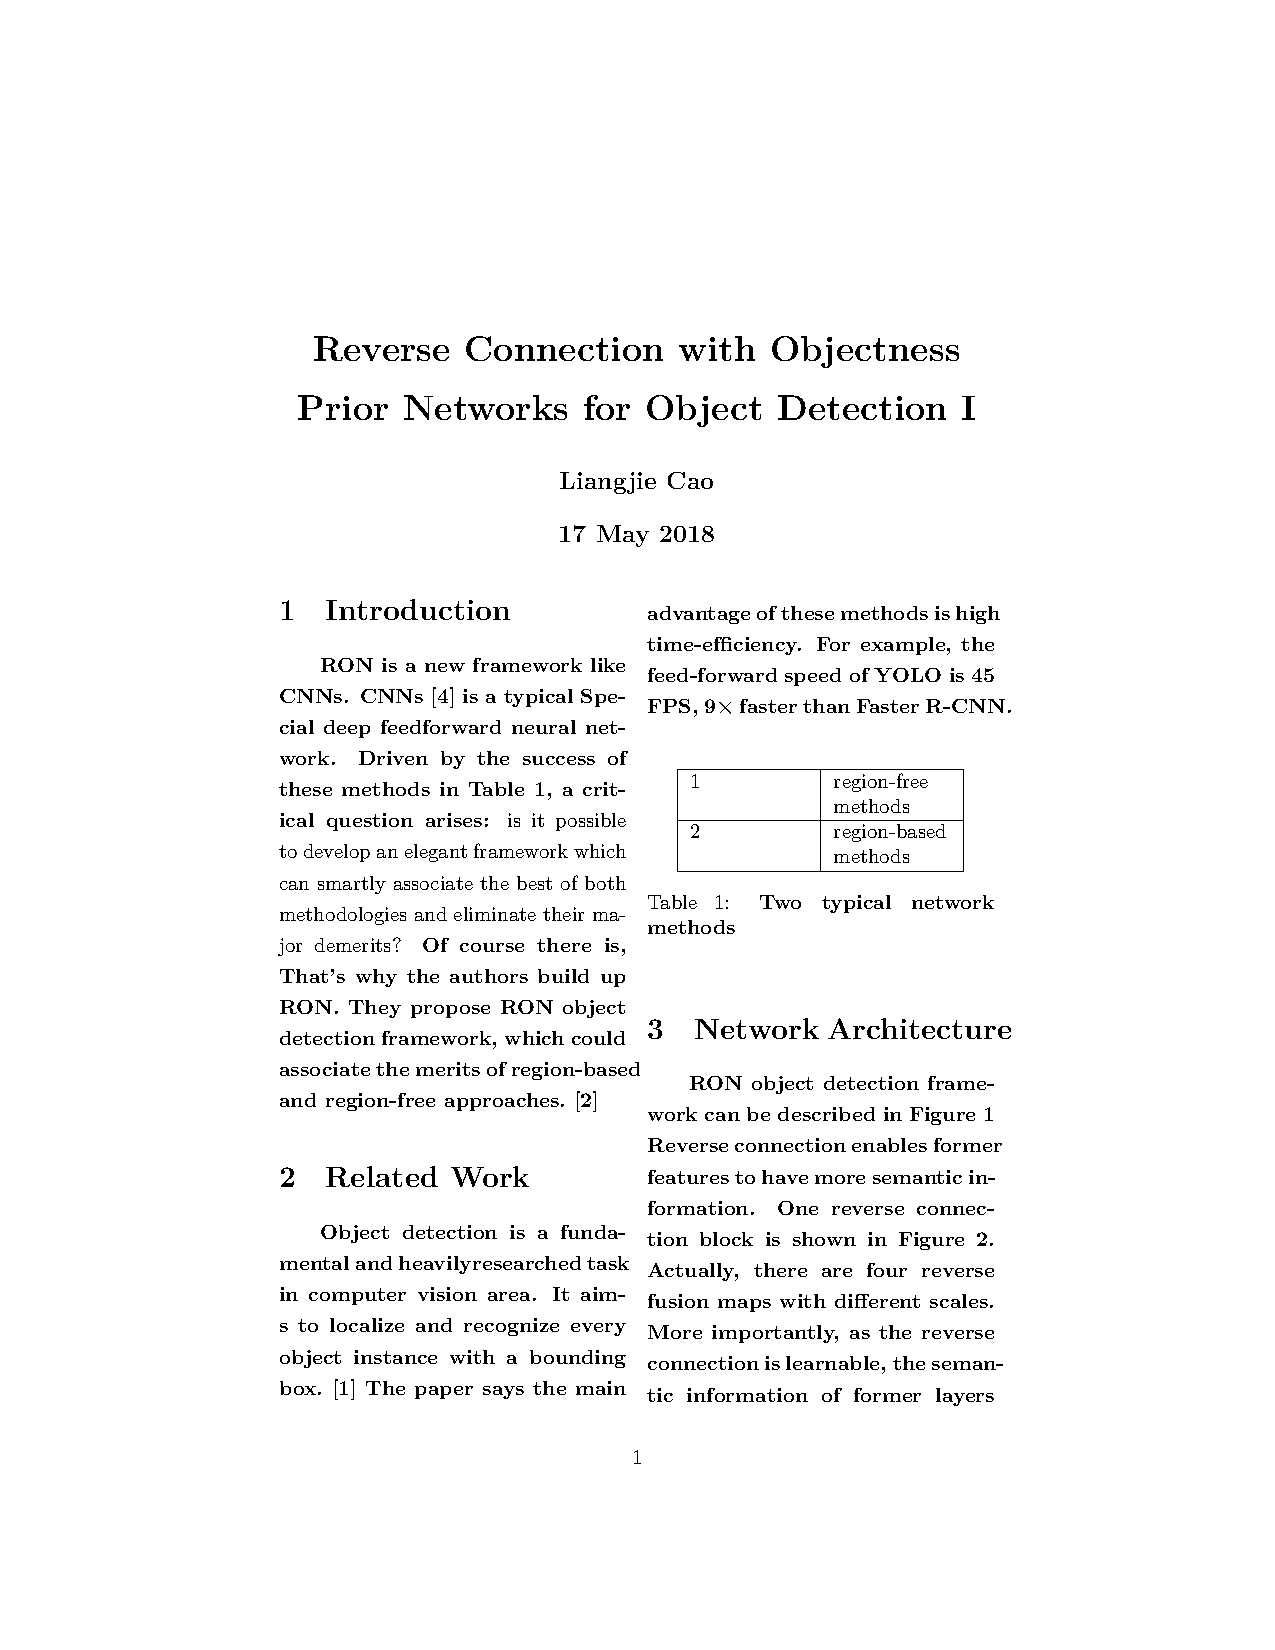
\includegraphics[width=0.5\textwidth]{RON.png}\\
 \caption{\textbf{RON object detection overview}}\label{Figure1}
  \centering
 \includegraphics[width=0.5\textwidth]{mod1.png}\\
 \caption{\textbf{ Objectness prior generated from a specific image.}}\label{Figure2}
\end{figure}
\par
\section{Objectness Prior}
\textbf{As shown in Section~\ref{Section 2}, they consider default boxes with different scales and aspect ratios from many feature maps. However, only a tiny fraction of boxes covers objects. In other words, the ratio between object and non-object samples is seriously imbalanced. Figure\ref{Figure2} shows the multi-scale objectness prior generated from a specific image. For visualization, the objectness prior maps are averaged along the channel dimension. We see that the objectness prior maps could explicitly reflect the existence of an object. And objects of various scales will respond at their corresponding feature maps, and we enable this by appropriate matching and end-to-end training.
}\\
\bibliographystyle{plain}
\bibliography{yinyong1}
\end{document}

